\documentclass{article}
\usepackage{longtable}
\usepackage{multirow}
\usepackage{array}
\documentclass{article}
\usepackage{graphicx}  % For inserting images
\usepackage{caption}   % For better caption formatting
\usepackage{float}     % To control figure placement


\title{Schema and Relationships}
\author{Eduardo Oliveira}
\date{\today}

\begin{document}

\maketitle

\section{Entities Representation}

\subsection{User Account}

\begin{longtable}{|l|l|p{8cm}|}
    \hline
    \multicolumn{1}{|c|}{\textbf{Entity}} & 
    \multicolumn{1}{c|}{\textbf{Attribute}} & 
    \multicolumn{1}{c|}{\textbf{Description}} \\
    \hline
    \multirow{2}{*}{\texttt{foaf:Person}}  
        & foaf:name & The name of the person. \\ \cline{2-3}
        & foaf:mbox & The email address of the person. \\ \cline{2-3} 
    \hline
    \multirow{3}{*}{\texttt{foaf:holdsAccount}}  
        & schema:identifier & The account name of the person in the blockchain. \\ \cline{2-3}
        & schema:roleName & The role of the person in the platform. \\ \cline{2-3}
        & schema:publicKey & The cryptographic public key of the account in the blockchain. \\ 
    \hline
    \multirow{1}{*}{\texttt{foaf:Organization}}  
        & foaf:name & The name of the organization the person belongs to. \\ \cline{1-3}
         
    \hline
    \multirow{2}{*}{\texttt{schema:identifier}}  
        & propertyID & The type of identifier is ORCID (Open Researcher and Contributor ID). \\ \cline{2-3}
        & value & The actual ORCID value for the person. \\ 
    \hline
    \end{longtable}
    
\subsection{Project Account}

\begin{longtable}{|l|l|p{8cm}|}
    \hline
    \multicolumn{1}{|c|}{\textbf{Entity}} & 
    \multicolumn{1}{c|}{\textbf{Attribute}} & 
    \multicolumn{1}{c|}{\textbf{Description}} \\
    \hline
    \multirow{3}{*}{\texttt{foaf:Person}}  
        & foaf:name & The name of the person. \\ \cline{2-3}
        & foaf:mbox & The email address of the person. \\ \cline{2-3}
        & foaf:holdsAccount & Links the person to an account. \\ 
    \hline
    \multirow{2}{*}{\texttt{foaf:Organization}}  
        & foaf:name & The name of the organization. \\ \cline{2-3}
        & foaf:location & The physical or digital location of the organization. \\ 
    \hline
    \multirow{2}{*}{\texttt{schema:identifier}}  
        & propertyID & The type of identifier (e.g., ORCID). \\ \cline{2-3}
        & value & The actual identifier value. \\ 
    \hline
    \end{longtable}


    \section{Entity-Relationship Diagram}

    The diagram below represents the relationships between various entities extracted from the given JSON-LD data. The main entities in the diagram include:
    
    \begin{itemize}
        \item \textbf{foaf:Person} – Represents an individual, identified by attributes such as name, email, and affiliation.
        \item \textbf{foaf:Organization} – Represents an institution or organization to which a person is affiliated.
        \item \textbf{foaf:holdsAccount} – Represents an individual's digital account, containing an identifier, role, and public key.
        \item \textbf{schema:identifier} – Represents a unique identifier (such as an ORCID) assigned to a person.
        \item \textbf{schema:linked_project} – Represents a research project associated with a specific individual.
    \end{itemize}
    
    
    Each \texttt{foaf:Person} entity is associated with an \texttt{foaf:Organization}, has a \texttt{foaf:holdsAccount}, and a unique \texttt{schema:identifier}. The entity "Upbeat Neumann" also has an additional relationship linking them to a specific research project.
    
    \vspace{1cm}
    
    \begin{figure}[H]
        \centering
        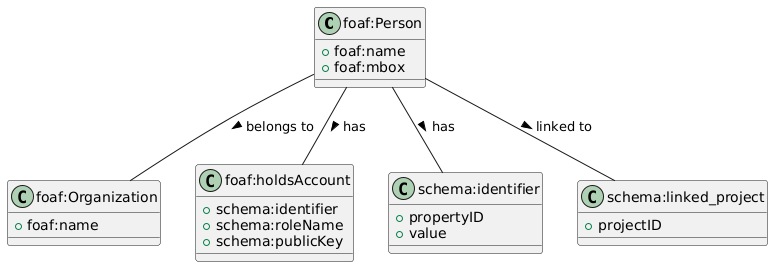
\includegraphics[width=\textwidth]{/home/eduardo/Documents/repo/Git/OpenScience/out/diagrams/plantUML/account/account.png}  % Placeholder for the SVG file
        \caption{Entity-Relationship Diagram foror the user account.}
        \label{fig:er-diagram}
    \end{figure}
    
    
\end{document}


